\resizebox{\textwidth}{!}{%
	\tikzstyle{connector} = [thick,->]
	\tikzstyle{block} = [draw,thick,rectangle,minimum height=2.5em,minimum width=2cm]
	\tikzstyle{blocklong} = [draw,thick,rectangle,minimum height=2.5em,minimum width=2.35cm]
	\tikzstyle{blockLong} = [draw,thick,rectangle,minimum height=3.5em,minimum width=6.3cm]
	
	\tikzstyle{nil} = [inner sep=0pt]
	\begin{tikzpicture}[>=latex',node distance=2.1cm,auto]
		\node (lefta) [nil] {};
		\node (imageNet) at (lefta) {\includegraphics[height=3.5em]{figures/EKGsmall}};
		\node (TrainData) [blockLong, left = -4.41cm of lefta] {};
		%        \node (LabelText) [right = of imageNet] {\scriptsize{Labels e.g. mat,}};
		\node (LabelText) at (3.11,0.3) {\scriptsize{Labels e.g. healty,}};
		\node (LabelText2) [below = 0cm of LabelText] {\scriptsize{art. fib., RBBB}};
		\node (TDtext) at (1, 1.0){Training data};
		
		\node (Model) [block] at (-1.1,-2) {Model};
		
		\node (LA) [blocklong] at (2.85,-2) {};
		\node (LAright) [right = 1cm of LA] {};
		\node (LAunderR) [below = 1.2cm of LAright] {};
		\node (Munder) [below = 1.0cm of Model] {};
		
		\node (LAText1) at (2.75,-1.8) {Learning};
		\node (LAText1) at (2.75,-2.2) {algorithm};
		
		\node (TDunderL) at (-1,-0.55) {};
		\node (ModelOver) at (-1,-1.67) {};
		\draw[connector] (TDunderL) -- (ModelOver) {};
		
		\node (TDunderR) at (2.8,-0.55) {};
		\node (LAOver) at (2.8,-1.67) {};
		\draw[connector] (TDunderR) -- (LAOver) {};
		
		\draw[connector] (Model) -- (LA) {};
		
		\draw[thick,-] (LA) -- (LAright) {};
		\draw[thick,-] (LAright.west) -- (LAunderR.west) {};
		\draw[thick,-] (LAunderR) -- (Munder.north) {};
		\draw[connector] (Munder) -- (Model.south) {};
		
		\node (PredictionText) at (0.75,-2.25) {\scriptsize{prediction}};
		\node (PredictionText) at (2,-3.25) {\scriptsize{update model}};		
	\end{tikzpicture}
	\qquad \qquad 
	\tikzstyle{blockLong} = [draw,thick,rectangle,minimum height=3.5em,minimum width=3.7cm]
	\begin{tikzpicture}[>=latex',node distance=2.1cm,auto]
		\node (lefta2) [nil] {};
		\node (imageNet2) [left = -0.2cm of lefta2] {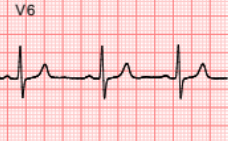
\includegraphics[height=3.5em]{figures/EKGpred}};
		\node (TrainData2) [blockLong, left = -1.6cm of lefta2] {};
		\node (LabelText) at (0.8,0) {?};
		\node (TDtext) at (-0.4, 1.0){Unseen data};
		
		\node (Model2) [block] at (-1.1,-2) {Model};
		
		\node (LA2) at (1.85,-2) {};
		
		\node (TDunderL2) at (-1,-0.55) {};
		\node (ModelOver2) at (-1,-1.67) {};
		\draw[connector] (TDunderL2) -- (ModelOver2) {};
		
		\draw[connector] (Model2) -- (LA2) {};
		
		\node (PredictionText) at (0.75,-2.25) {\scriptsize{prediction}};
	\end{tikzpicture}

	}